\section{Replication on biological breast tissue and segmentation context}\label{sec:external-validation}
\subsection{Data and selection}
We used the public 10x FFPE Human Breast with Pre-designed Panel dataset, processed with Xenium Onboard Analysis 1.0.2~\cite{biologicalbreast}. It contains an infiltrating ductal carcinoma sample with ductal carcinoma in situ and an invasive lobular carcinoma sample from two donors. Both are distinct tissue sources from the lung donor. The donor identity behind the earlier breast format-test input is unspecified, so we make no claim that it supplies an additional independent breast donor. The new sources use DAPI nuclear segmentation and vendor expansion by $15\,\mu\mathrm m$; their native cell masks define the reference partitions.

For each donor, we formed three target locations using the 25th, 50th and 75th percentiles of cell-centroid $x$ and the median cell-centroid $y$. The nearest cell centroid to each target fixed a nominal $200\times200\,\mu\mathrm m$ core and an $800\times800\,\mu\mathrm m$ context window. Origins were rounded down to the native pixel grid. The selection used no gene identities, transcript counts or GeoCert outcomes. All six cores were retained. Their coordinates, source-member checksums and selection rules are recorded with the analysis.

\begin{figure}[ht]\centering
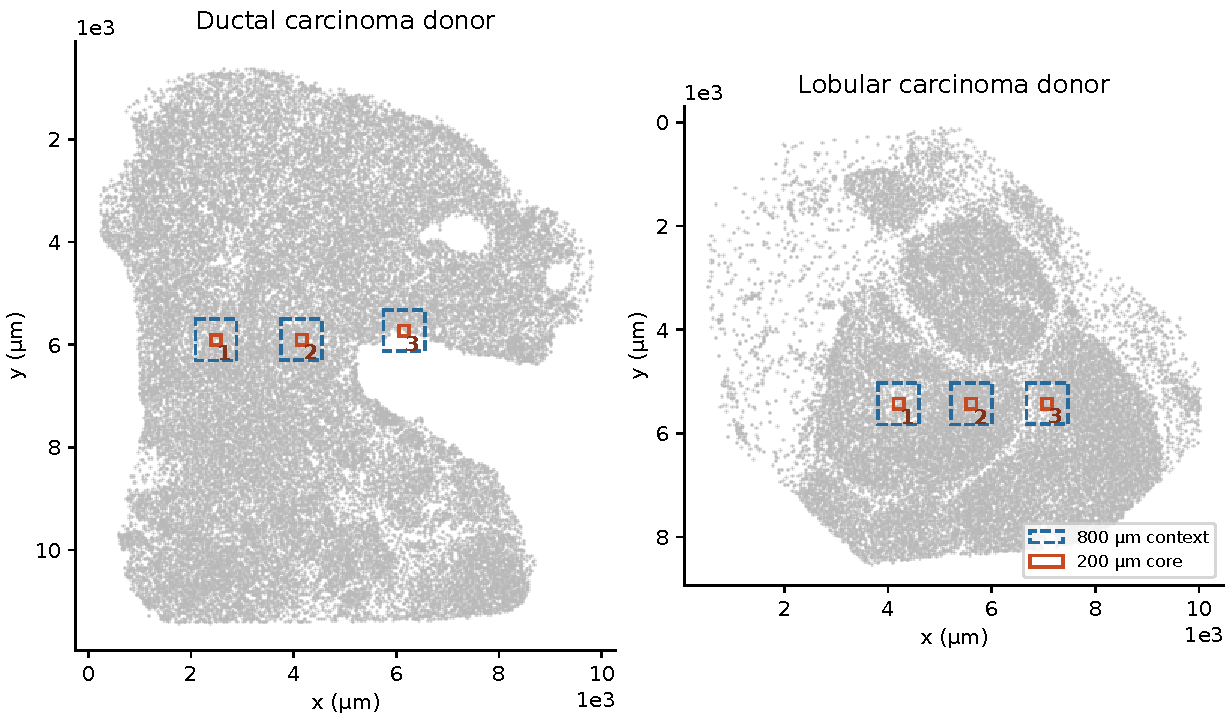
\includegraphics[width=.95\textwidth]{figures/biological_regions.pdf}
\caption{The six predefined breast tissue regions. Grey points show a regularly subsampled set of source cell centroids; solid boxes mark the analysis cores and dashed boxes the surrounding Proseg inputs. Each panel represents one donor.}\label{fig:biological-regions}
\end{figure}

The original cell and nucleus raster masks, physical coordinate transform and transcript identifiers were retained. We included every Q20 transcript targeting a measured gene in the selected regions. An independent pass through the original Parquet files reproduced all retained identifiers, coordinates, raster assignments and source counts. There were zero discrepancies between retained transcript owners and the native masks. Cells touching a core edge or lacking a connected valid reference region were excluded by the unchanged atlas eligibility rule.

\FloatBarrier
\subsection{Exact count intervals and matched approximations}
The primary atlas uses the original ribbon-width ladder, slope, nuclear constraints and fixed seams, with the original eight area budgets. Questions cover positive or editable cell--gene pairs, retaining the fixed counts outside ribbons. Extraction and independent rational checks precede count computation. We used exact implication-pruned enumeration for local single-gene spectra; every spectrum completed. Separate scalar calculations reproduced all local minima, and Cartesian composition and explicit boundary checks verified every global spectrum and endpoint. The analysis therefore tests the existing model on new biological samples without changing its geometric assumptions.

\begin{table}[ht]\centering
\begin{tabular}{lrr}\toprule
Quantity&Ductal donor&Lobular donor\\\midrule
Complete eligible cells&659&859\\
Retained core transcripts&97,893&91,659\\
Boundary ribbons&1,531&1,946\\
Covered eligible shared edges&76.5\%&76.5\%\\
Cell--gene questions&32,360&36,409\\
Invariant at $4\,\mu\mathrm m^2$&25,749 (79.6\%)&30,403 (83.5\%)\\
Questions with outer width at least two&1,271&829\\
Questions tightened by shared geometry&176 (13.8\%)&97 (11.7\%)\\
Questions with an additive missed endpoint&58&37\\\bottomrule
\end{tabular}
\caption{Results across three predefined cores per donor. Invariance is conditional on the primary atlas's approximately $0.45\,\mu\mathrm m$ displacement cap and fixed uncovered boundaries. Eligibility, tightening and additive misses are counted once per cell--gene question across the eight budgets. Tightening affects 0.54\% and 0.27\% of all questions, respectively.}\label{tab:biological-replication}
\end{table}

The independent-molecule outer bound uses the same exact singleton transfer costs as the original analysis. The additive inner approximation retains assignment feasibility while replacing shared area by the sum of singleton costs, including collateral transfers. These comparisons separate the effects of shared geometry and shared deformation cost. A further distance-only outer bound counts molecules near raster boundary edges using the global displacement cap and a half-pixel allowance for representing each unit edge by its midpoint. It relaxes the ribbon, nuclear and area constraints; tightening against that looser bound alone is not evidence of a shared-cost effect.

\begin{table}[ht]\centering
\begin{tabular}{rrrrr}\toprule
Budget ($\mu\mathrm m^2$)&\multicolumn{2}{c}{Ductal donor}&\multicolumn{2}{c}{Lobular donor}\\
&Non-singleton&Tighter outer&Non-singleton&Tighter outer\\\midrule
0&0&0&0&0\\
0.05&5,082&94&4,551&40\\
0.1&5,770&62&5,249&43\\
0.25&6,611&38&6,006&17\\
0.5&6,611&0&6,006&0\\
1&6,611&0&6,006&0\\
2&6,611&0&6,006&0\\
4&6,611&0&6,006&0\\\bottomrule
\end{tabular}
\caption{Budget-specific counts in the two biological donors. The shared-geometry differences occur at smaller budgets; the singleton outer bounds coincide with the exact intervals from $0.5\,\mu\mathrm m^2$ onward on this grid.}
\end{table}

\FloatBarrier
\subsection{Paired Proseg context analysis}
For each breast core and both original lung crops, we ran Proseg 3.2.0 on the core alone and with $300\,\mu\mathrm m$ of surrounding tissue on each side. Default factorization and the earlier no-factorization setting were tested separately, keeping 200 burn-in iterations, 200 sampling iterations, 50 hill-climbing iterations and two threads. The default run on the first small lung crop again failed; it was retained as a failed setting rather than replaced. Each completed setting is one stochastic run, so differences are descriptive and include sampling variability.

Comparisons use the same original core transcript identifiers retained by all completed settings for that core, with output cell identities joined to source identities. Background assignments override the reported cell index. We reconcile final transcript assignments from the native Proseg Parquet output with its sparse count matrix; optional CSV exports are not required for this check. All settings for a core use the union of their source and alternative cell--gene questions. Queries affected by an excluded editable transcript are marked unavailable rather than scored with a shifted full-transcript spectrum. We report cell-to-cell transfers and background transfers separately. Countwise inclusion in an interval is distinguished from realizability of the complete assignment vector.

\begin{table}[ht]\centering\small
\begin{tabular}{lrrrrr}\toprule
Core&Retained/input RNA&\multicolumn{2}{c}{Default factorization}&\multicolumn{2}{c}{No factorization}\\
&&$200\,\mu\mathrm m$&$800\,\mu\mathrm m$&$200\,\mu\mathrm m$&$800\,\mu\mathrm m$\\\midrule
LUNG 1&5,774/5,847&failed&19.5&42.5&19.4\\
LUNG 2&1,482/1,523&86.5&60.7&89.8&62.1\\
IDC 1&27,250/27,250&29.2&21.3&29.3&21.0\\
IDC 2&45,198/45,198&24.2&14.8&24.0&15.1\\
IDC 3&25,329/25,445&27.9&12.5&27.9&12.2\\
ILC 1&22,791/22,791&27.7&16.6&28.8&16.6\\
ILC 2&41,168/41,168&20.1&9.8&19.8&9.7\\
ILC 3&27,700/27,700&27.1&13.8&28.2&14.0\\
\bottomrule\end{tabular}
\caption{Percentage of retained core transcripts assigned to background. Each row uses the intersection of core transcript identifiers across completed settings; the second column reports its size against the original core input. Input width describes the surrounding window, while evaluation always uses the central core.}\label{tab:context-background}
\end{table}
\begin{table}[ht]\centering\small
\begin{tabular}{llrrrr}\toprule
Core&Setting&Changed counts&Reach (\%)&With BG (\%)&Fixed RNA moves\\\midrule
LUNG 1&200 / D&\multicolumn{4}{c}{Factorization failed}\\
LUNG 1&200 / NF&2,262&7.2&68.0&2,777\\
LUNG 1&800 / D&2,198&8.2&39.4&2,292\\
LUNG 1&800 / NF&2,139&7.8&40.0&2,347\\
LUNG 2&200 / D&513&5.1&90.4&683\\
LUNG 2&200 / NF&504&5.2&95.4&684\\
LUNG 2&800 / D&433&5.3&75.1&519\\
LUNG 2&800 / NF&470&4.9&75.3&571\\
IDC 1&200 / D&7,113&7.1&60.3&11,280\\
IDC 1&200 / NF&7,048&6.9&61.3&11,226\\
IDC 1&800 / D&6,496&7.9&45.7&9,572\\
IDC 1&800 / NF&6,541&7.9&45.3&9,473\\
IDC 2&200 / D&11,107&7.9&57.0&17,495\\
IDC 2&200 / NF&11,094&7.8&56.4&17,549\\
IDC 2&800 / D&10,059&9.2&37.0&14,560\\
IDC 2&800 / NF&10,126&9.1&38.1&14,597\\
IDC 3&200 / D&6,226&8.4&66.1&10,321\\
IDC 3&200 / NF&6,363&7.8&66.0&10,286\\
IDC 3&800 / D&5,660&9.8&33.8&7,794\\
IDC 3&800 / NF&5,570&10.3&34.1&7,689\\
ILC 1&200 / D&6,558&6.8&62.3&8,951\\
ILC 1&200 / NF&6,662&6.6&62.9&9,073\\
ILC 1&800 / D&5,729&8.0&41.1&6,897\\
ILC 1&800 / NF&5,801&8.0&41.3&6,862\\
ILC 2&200 / D&10,975&8.2&51.8&14,360\\
ILC 2&200 / NF&11,021&8.5&50.9&14,446\\
ILC 2&800 / D&9,699&9.6&27.7&11,234\\
ILC 2&800 / NF&9,651&9.9&26.9&11,202\\
ILC 3&200 / D&8,166&6.1&61.3&10,366\\
ILC 3&200 / NF&8,240&5.9&62.6&10,626\\
ILC 3&800 / D&7,227&7.2&35.5&7,768\\
ILC 3&800 / NF&7,297&7.0&35.7&7,838\\
\bottomrule\end{tabular}
\caption{All paired Proseg settings. D: default factorization; NF: no factorization. Reach is the fraction of changed cell--gene counts individually attainable within the primary atlas at $4\,\mu\mathrm m^2$. With BG counts changed entries touched by at least one transfer to or from background; these may also involve cell-to-cell transfers. Fixed RNA moves count reassigned transcripts outside editable ribbons. Every completed full assignment lies outside the family. Each core uses a fixed set of cell--gene questions across its completed settings.}\label{tab:context-reach}
\end{table}
\FloatBarrier
In the original lung cores, the matched no-factorization background fractions change from 42.5\% to 19.4\% and from 89.8\% to 62.1\% when surrounding tissue is included. Thus the extreme background rates in the small-crop comparison depend on the input context. Larger inputs still produce many changes outside the primary family (Table~\ref{tab:context-reach}). These results diagnose the comparison setting; they do not establish which assignments are anatomically correct or isolate context effects from stochastic variability.

The public artifacts retain core transcript assignments for every completed run, the complete setting inventory, countwise comparisons and audit results. Replaying those extracts reproduces the tables; repeating Proseg itself is stochastic. Native transcript outputs were reconciled with the full output count matrices before the core extracts were saved.

